\section{Truss Direct Stiffness Method}

% Direct Stiffness Method Resource:
% https://www.colorado.edu/engineering/CAS/Felippa.d/FelippaHome.d/Publications.d/Report.CU-CAS-00-13.pdf

%Assumptions: In a truss external loading is only applied to the joints and there is only axial deformation with no bending.

The \textit{Direct Stiffness Method} is a \textit{Finite Element Method} of analysis that models structural elements as springs. We will begin with deriving the axial stiffness of a structural element. \cite{Felippa2000}

\subsection{Axial Stiffness}
Members in a truss are modelled as springs with only axial deformation. The axial force in the spring is modelled by Hooke's law:

\begin{equation}
	F = k u
\end{equation}

where $F$ is the axial force, $k$ is the axial stiffness, and $u$ is the axial deformation. To define the axial stiffness we will look at a member of constant cross-secitonal area with only elastic deformation. The stress in such a member is defined by the stress-strain relationship:

\begin{equation}
	\sig = E \ep
\end{equation}

where $\sig$ is the stress, $E$ is the modulus of elasticity, and $\ep$ is the strain. Multiplying both sides of the equation by the cross-secional area, $A$, will convert the stress into a force.

\begin{align}
	\sig A &= E \ep A\\
	F & = E \ep A
\end{align}

The engineering definition of strain will be used here. Strain is defined as:

\begin{equation}
	\ep = \frac{\Delta L}{L_0} = \frac{u}{L}
\end{equation}

where $L$ is the original length of the member and $\Delta L$ is the change in length of the member. Then substituting in the definition of engineering strain into the previous equation:

\begin{align}
	F & = EA \frac{u}{L}
\end{align}

Therefore the axial stiffness from the equation is $\frac{AE}{L}$ for any structural member. The axial force of a structural element can be rewritten as:

\begin{align}
	F & = \frac{AE}{L} u
\end{align}

\subsection{Local Element Stiffness}
Each element in a structural system will have its own local element stiffness equations. The goal of this section will be to develop the local element stiffness equations for a member in matrix form. Taking the nodal equilibrium from figure \ref{fig:LocalMemberStiffness} becomes:

\begin{align*}
	-F &= ku_{1x'}\\
	-F &= ku_{2x'}\\
\end{align*}

Next we will put these equations in matrix form in terms of the local coordinate system. The equation will take the form:

\begin{equation}
	\vec{F} = \vec{k} \vec{u}
\end{equation}

\begin{center}
	\begin{figure}[h]	\centerline{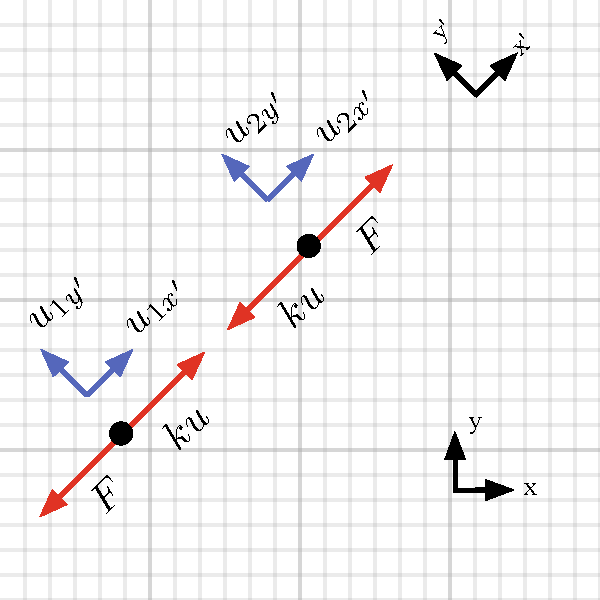
\includegraphics[width=0.7\columnwidth]{Figures/LocalMemberStiffness}}
		\caption{Local Member FBDs}
		\label{fig:LocalMemberStiffness}
	\end{figure}
\end{center}


\begin{equation}
	\begin{bmatrix}
	-F\\ 0\\ F\\ 0\\
	\end{bmatrix}
	=
	\frac{AE}{L}
	\begin{bmatrix}
	1 & 0 & -1 & 0\\
	0 & 0 & 0 & 0\\
	-1 & 0 & 1 & 0\\
	0 & 0 & 0 & 0\\
	\end{bmatrix}
	\begin{Bmatrix}
	u_{1x'}\\ u_{1y'}\\ u_{2x'}\\ u_{2y'}\\
	\end{Bmatrix}
\end{equation}

Next, we must take the local element stiffness matrix and derive the global element stiffness matrix.

\subsection{Global Element Stiffness}


\subsection{Global Structural Stiffness}


%Boundary Conditions

